% ============================================================
%  يُترجَم بـ XeLaTeX  (في Overleaf: Menu → Compiler → XeLaTeX)
%  الخط: Amiri (متوفر في Overleaf، أو حمّله من github.com/aliftype/amiri)
% ============================================================
\documentclass[12pt,a4paper]{article}
\usepackage[a4paper,margin=1.7cm,top=2.3cm,bottom=2.9cm,headheight=15pt,footskip=1.5cm]{geometry}
\usepackage{amsmath,amssymb}
\usepackage{icomma}
\usepackage[english,bidi=default,layout=lists]{babel}
\babelprovide[import,main]{arabic}
\babelfont{rm}[Scale=1.08]{Amiri}
\babelfont{sf}[Scale=1.08]{Amiri}
\usepackage[most]{tcolorbox}
\usepackage{tikz}
\usetikzlibrary{arrows.meta,calc,shadings}
\usepackage{array}
\usepackage{colortbl}
\usepackage{fancyhdr}
\usepackage{titlesec}
\usepackage{enumitem}
\usepackage{collcell}
\usepackage{needspace}
\usepackage{etoolbox}
\newcolumntype{C}{>{\collectcell\ar}c<{\endcollectcell}}
\pretocmd{\section}{\Needspace{15\baselineskip}}{}{}
\pretocmd{\subsection}{\Needspace{11\baselineskip}}{}{}

\definecolor{cDef}{HTML}{1F4E9C}
\definecolor{cThm}{HTML}{B3261E}
\definecolor{cRem}{HTML}{2E7D32}
\definecolor{cEx}{HTML}{C76B00}
\definecolor{cMeth}{HTML}{6A1B9A}
\definecolor{cSol}{HTML}{00695C}
\definecolor{cSec}{HTML}{1F3A68}

\titleformat{\section}{\Large\bfseries\color{cSec}}{\thesection.}{0.6em}{}[{\color{cSec!60}\titlerule[1pt]}]
\titleformat{\subsection}{\large\bfseries\color{cThm!85!black}}{\thesubsection.}{0.5em}{}
\titlespacing*{\section}{0pt}{14pt}{8pt}
\titlespacing*{\subsection}{0pt}{10pt}{5pt}
\setlength{\parindent}{0pt}
\setlength{\parskip}{4pt}
\setlist{itemsep=2pt,topsep=3pt}

\newtcolorbox{arbox}[3][]{enhanced,
  colback=#2!5,colframe=#2!80!black,arc=2mm,boxrule=0.8pt,
  left=6pt,right=6pt,top=8pt,bottom=5pt,
  fonttitle=\bfseries,coltitle=white,
  title={\foreignlanguage{arabic}{#3}},
  attach boxed title to top right={xshift=-5mm,yshift=-3mm},
  boxed title style={colback=#2!80!black,arc=1.5mm,boxrule=0pt},
  before upper={\selectlanguage{arabic}},
  before skip=8pt,after skip=8pt,breakable,#1}
\newenvironment{BOX}[2]{\begin{otherlanguage}{english}\begin{arbox}{#1}{#2}}{\end{arbox}\end{otherlanguage}}
\newenvironment{tarif}[1][تعريف]{\begin{BOX}{cDef}{#1}}{\end{BOX}}
\newenvironment{khassia}[1][خاصية]{\begin{BOX}{cThm}{#1}}{\end{BOX}}
\newenvironment{molahada}[1][ملاحظة]{\begin{BOX}{cRem}{#1}}{\end{BOX}}
\newenvironment{mithal}[1][مثال]{\begin{BOX}{cEx}{#1}}{\end{BOX}}
\newenvironment{tariqa}[1][طريقة]{\begin{BOX}{cMeth}{#1}}{\end{BOX}}

\newcounter{exo}
\newenvironment{tamrin}[1]{\stepcounter{exo}\begin{BOX}{cSec}{التمرين \theexo: #1}}{\end{BOX}}
\newenvironment{hal}{\Needspace{12\baselineskip}\begin{otherlanguage}{english}\begin{arbox}[breakable]{cSol}{حل التمرين \theexo}}{\end{arbox}\end{otherlanguage}}

\newenvironment{LTR}{\begin{otherlanguage}{english}}{\end{otherlanguage}}
\newcommand{\ar}[1]{\foreignlanguage{arabic}{#1}}

\renewcommand{\dots}{\mathinner{\ldotp\ldotp\ldotp}}
\renewcommand{\ldots}{\mathinner{\ldotp\ldotp\ldotp}}
\renewcommand{\cdots}{\mathinner{\cdotp\cdotp\cdotp}}
\newcommand{\N}{\mathbb{N}}
\newcommand{\Z}{\mathbb{Z}}
\newcommand{\D}{\mathbb{D}}
\newcommand{\Q}{\mathbb{Q}}
\newcommand{\R}{\mathbb{R}}
\newcommand{\pgcd}{\operatorname{PGCD}}
\newcommand{\ppcm}{\operatorname{PPCM}}

% \NLseg{a}{b}{[}{]} ; \NLright{a}{[} ; \NLleft{b}{]}  (interval on a number line)
\newcommand{\NLseg}[4]{\begin{LTR}\begin{tikzpicture}[baseline=-0.6ex]
 \draw[-{Stealth[length=2mm]},gray!70](0,0)--(3.4,0);
 \draw[line width=2pt,cThm!80!black](0.7,0)--(2.7,0);
 \node[cThm!80!black,font=\LARGE] at (0.7,0){$#3$};
 \node[cThm!80!black,font=\LARGE] at (2.7,0){$#4$};
 \node[below=3pt,font=\footnotesize] at (0.7,0){$#1$};
 \node[below=3pt,font=\footnotesize] at (2.7,0){$#2$};
\end{tikzpicture}\end{LTR}}
\newcommand{\NLright}[2]{\begin{LTR}\begin{tikzpicture}[baseline=-0.6ex]
 \draw[-{Stealth[length=2mm]},gray!70](0,0)--(3.4,0);
 \draw[line width=2pt,cThm!80!black](1.3,0)--(3.3,0);
 \node[cThm!80!black,font=\LARGE] at (1.3,0){$#2$};
 \node[below=3pt,font=\footnotesize] at (1.3,0){$#1$};
\end{tikzpicture}\end{LTR}}
\newcommand{\NLleft}[2]{\begin{LTR}\begin{tikzpicture}[baseline=-0.6ex]
 \draw[-{Stealth[length=2mm]},gray!70](0,0)--(3.4,0);
 \draw[line width=2pt,cThm!80!black](0.05,0)--(2.1,0);
 \node[cThm!80!black,font=\LARGE] at (2.1,0){$#2$};
 \node[below=3pt,font=\footnotesize] at (2.1,0){$#1$};
\end{tikzpicture}\end{LTR}}

% ---------- social-media icons (pure TikZ) ----------
\definecolor{cFB}{HTML}{1877F2}
\definecolor{cTG}{HTML}{229ED9}
\definecolor{cIG1}{HTML}{FEDA75}
\definecolor{cIG2}{HTML}{D62976}
\definecolor{cIG3}{HTML}{4F5BD5}
\newcommand{\fbicon}{\begin{LTR}\begin{tikzpicture}[baseline=-0.75ex,x=1em,y=1em]
 \fill[cFB] (0,0) circle (0.55);
 \node[white,inner sep=0,font=\usefont{TU}{lmss}{bx}{n}\small] at (0.04,-0.02) {f};
\end{tikzpicture}\end{LTR}}
\newcommand{\igicon}{\begin{LTR}
\begin{tikzpicture}[baseline=-0.75ex,x=1em,y=1em]
 \shade[lower left=cIG1,lower right=cIG2,upper left=cIG2,upper right=cIG3,rounded corners=0.28em] (-0.55,-0.55) rectangle (0.55,0.55);
 \draw[white,line width=0.09em,rounded corners=0.18em] (-0.36,-0.36) rectangle (0.36,0.36);
 \draw[white,line width=0.09em] (0,0) circle (0.17);
 \fill[white] (0.22,0.22) circle (0.05);
\end{tikzpicture}\end{LTR}}
\newcommand{\tgicon}{\begin{LTR}
\begin{tikzpicture}[baseline=-0.75ex,x=1em,y=1em]
 \fill[cTG] (0,0) circle (0.55);
 \fill[white] (-0.33,0.0) -- (0.32,0.27) -- (0.2,-0.3) -- (0.0,-0.15) -- (-0.08,-0.28) -- (-0.08,-0.08) -- cycle;
 \fill[cTG!70!black] (-0.08,-0.08) -- (0.25,0.2) -- (0.0,-0.15) -- (-0.08,-0.28) -- cycle;
\end{tikzpicture}\end{LTR}}
% page number: black box, white two-digit number, at the right of the social row
\newcommand{\PageBox}{\begin{LTR}\tikz[baseline=(p.base)]\node[fill=black,text=white,inner sep=2.5pt,minimum width=1.6em,minimum height=1.3em,font=\usefont{TU}{lmss}{bx}{n}\small](p){\ifnum\value{page}<10 0\fi\arabic{page}};\end{LTR}}
% visual left-to-right order: Telegram | Instagram | Facebook | page box
\newcommand{\SocialRow}{\begin{otherlanguage}{english}%
 \ar{\textbf{الأستاذ سوايسية هشام للرياضيات}}\ \tgicon\hfill
 \textbf{prof\_hicham\_math}\ \igicon\hfill
 \ar{\textbf{الأستاذ سوايسية هشام للرياضيات}}\ \fbicon\hspace{2.2em}\PageBox\end{otherlanguage}}

\pagestyle{fancy}
\fancyhf{}
\renewcommand{\headrulewidth}{0.6pt}
\renewcommand{\footrulewidth}{0.4pt}
% \SetHeader{right head: document title}{left head: level -- stream}
\newcommand{\SetHeader}[2]{%
 \fancyhead[C]{\parbox{\textwidth}{\ar{#1\hfill #2}}}%
 \fancyfoot[C]{\parbox{\textwidth}{\small\SocialRow}}}
\usepackage{tkz-tab}
\usepackage{multicol}
% variation / sign table (LTR)
\newenvironment{TAB}{\par\begin{center}\begin{LTR}\begin{tikzpicture}[scale=0.95,every node/.style={font=\small}]}{\end{tikzpicture}\end{LTR}\end{center}}
% grid + axes, clipped: \begin{GR}{xmin}{xmax}{ymin}{ymax}{unit cm}
\newenvironment{GR}[5]{\par\begin{center}\begin{LTR}\begin{tikzpicture}[x=#5cm,y=#5cm,font=\footnotesize]
 \draw[gray!25,very thin] (#1,#3) grid (#2,#4);
 \draw[-{Stealth[length=2mm]}] (#1,0)--(#2+0.3,0) node[below left]{$x$};
 \draw[-{Stealth[length=2mm]}] (0,#3)--(0,#4+0.3) node[below left]{$y$};
 \node[below left] at (0,0){$O$};
 \begin{scope}\clip (#1,#3) rectangle (#2,#4);}
{\end{scope}\end{tikzpicture}\end{LTR}\end{center}}
\newcommand{\Ticks}[2]{\foreach \t in {#1} \node[below,font=\scriptsize] at (\t,0){$\t$}; \foreach \t in {#2} \node[left,font=\scriptsize] at (0,\t){$\t$};}
\newcommand{\bx}[1]{\ensuremath{\colorbox{cDef!12}{$\displaystyle #1$}}}
\newcommand{\TwoCol}[4]{\par\begin{LTR}\noindent\begin{minipage}[t]{#1\textwidth}\selectlanguage{arabic}#2\end{minipage}\hfill\begin{minipage}[t]{#3\textwidth}\selectlanguage{arabic}#4\end{minipage}\end{LTR}\par}
\newcommand{\RL}[4]{\TwoCol{#3}{#4}{#1}{#2}}  % \RL{w1}{right content}{w2}{left content}
\newcommand{\ok}{$\textcolor{cRem}{\checkmark}$}
\newcommand{\limn}{\displaystyle\lim_{n\to+\infty}}
% sub-questions, each on its own line
\newenvironment{sq}{\begin{itemize}[leftmargin=2.4em,itemsep=3pt]}{\end{itemize}}
\newcommand{\qa}{\item[(أ)]}\newcommand{\qb}{\item[(ب)]}\newcommand{\qc}{\item[(جـ)]}\newcommand{\qd}{\item[(د)]}\newcommand{\qe}{\item[(هـ)]}
\newcommand{\pa}{\par\smallskip\textbf{(أ)} }\newcommand{\pb}{\par\smallskip\textbf{(ب)} }\newcommand{\pc}{\par\smallskip\textbf{(جـ)} }\newcommand{\pd}{\par\smallskip\textbf{(د)} }\newcommand{\pe}{\par\smallskip\textbf{(هـ)} }
\newcommand{\QQ}[1]{\par\smallskip\textbf{#1.} }
\newenvironment{tmr}{\stepcounter{exo}\begin{BOX}{cSec}{تمرين محلول \theexo}}{\end{BOX}}
\newcommand{\ABC}[3]{\\[2pt]\begin{tabular}{p{0.28\textwidth}p{0.28\textwidth}p{0.28\textwidth}}(جـ) \ #3 & (ب) \ #2 & (أ) \ #1\end{tabular}}
\pretocmd{\section}{\Needspace{24\baselineskip}}{}{}
\newtcbox{\bxtbox}{on line,colback=cDef!12,colframe=cDef!12,boxrule=0pt,arc=1pt,boxsep=0pt,left=2pt,right=2pt,top=1pt,bottom=1pt}
\newcommand{\bxt}[1]{\foreignlanguage{english}{\bxtbox{\ar{#1}}}}
\usepackage{longtable}
\setlength{\LTpre}{4pt}\setlength{\LTpost}{0pt}
\newcommand{\Phase}[1]{\textbf{#1}}
\newcommand{\Fld}[2]{\textbf{#1:}\ #2}
% رأس المذكرة على نمط النموذج: إطار بعنوان «مذكرة رقم»، معلومات الحصة، ثم إطار الكفاءات
\newcommand{\ModhHead}[9]{%
\begin{LTR}
\begin{tcolorbox}[enhanced,colback=white,colframe=cThm!85!black,arc=4mm,boxrule=1pt,top=14pt,bottom=6pt,left=8pt,right=8pt,
 overlay={\node[fill=cThm!85!black,text=white,rounded corners=3mm,inner xsep=14pt,inner ysep=4pt,font=\large\bfseries] at ([yshift=0pt]frame.north){\ar{مذكرة رقم #1}};},
 before upper={\selectlanguage{arabic}}]
\begin{tabular}{@{}p{0.4\linewidth}p{0.55\linewidth}@{}}
\Fld{المستوى}{#2} & \Fld{الثانوية}{\dotfill}\\[3pt]
\Fld{المادة}{رياضيات} & \Fld{ميدان التعلم}{#3}\\[3pt]
\Fld{المدة}{#5} & \Fld{الوحدة التعلمية}{#4}\\[3pt]
\Fld{الأستاذ}{\dotfill} & \Fld{المحتوى المعرفي}{#6}\\
\end{tabular}
\end{tcolorbox}
\begin{tcolorbox}[enhanced,colback=white,colframe=cThm!85!black,arc=3mm,boxrule=0.8pt,sidebyside,sidebyside align=top,lefthand ratio=0.5,
 segmentation style={dashed,cThm!60},before upper={\selectlanguage{arabic}},before lower={\selectlanguage{arabic}}]
\textbf{الكفاءات المستهدفة:}\par #8
\tcblower
\textbf{الكفاءات القبلية:}\par #7
\end{tcolorbox}
\end{LTR}
\par\smallskip\textbf{الوسائل:} #9\par\smallskip}
\newenvironment{Sayr}{%
\begin{LTR}\renewcommand{\arraystretch}{1.25}
\begin{longtable}{|p{0.17\textwidth}|>{\centering\arraybackslash}p{0.06\textwidth}|p{0.53\textwidth}|>{\centering\arraybackslash}p{0.12\textwidth}|}
\hline\rowcolor{cThm!12}\ar{\textbf{توجيهات وتعاليق}} & \ar{\textbf{المدة}} & \ar{\textbf{سير الحصة}} & \ar{\textbf{مراحل الحصة}}\\\hline\endhead
\hline\endfoot}{\end{longtable}\end{LTR}}
% سطر في الجدول: \Row{مرحلة}{سير}{مدة}{توجيهات}
\newcommand{\Row}[4]{\ar{\small #4} & \ar{#3} & \ar{#2} & \cellcolor{cThm!8}\ar{\Phase{#1}}\\\hline}

\newcommand{\Lab}[2]{\foreignlanguage{english}{\tcbox[on line,colback=#1,colframe=#1,boxrule=0pt,arc=2pt,boxsep=1pt,left=5pt,right=5pt,top=1pt,bottom=1pt]{\ar{\textcolor{white}{\textbf{#2}}}}}}
\newcommand{\Num}[1]{\foreignlanguage{english}{\tikz[baseline=(c.base)]\node[fill=cDef,text=white,inner sep=2pt,font=\footnotesize\bfseries](c){#1};}}
\newcommand{\ck}{\ensuremath{{\color{cRem}\checkmark}}}
\newenvironment{Kad}[1]{\par\smallskip\Lab{#1}}{\par}
\SetHeader{\small\bfseries\color{cSec}مذكرات محور: الأعداد والحساب}{\small\color{cSec}السنة الأولى ثانوي -- جذع مشترك علوم وتكنولوجيا}
\begin{document}
\begin{LTR}
\begin{tcolorbox}[enhanced,colback=cThm!85!black,colframe=cThm!85!black,arc=3mm,halign=center,boxrule=0pt,top=12pt,bottom=12pt,before upper={\selectlanguage{arabic}}]
{\color{white}\fontsize{26}{32}\selectfont\bfseries مذكرات محور: الأعداد والحساب}\\[8pt]
{\color{white}\large السنة الأولى ثانوي -- جذع مشترك علوم وتكنولوجيا}\\[4pt]
{\color{white}\large 11 مذكرة (22 ساعة) -- السنة الدراسية 2026-2027}
\end{tcolorbox}
\end{LTR}
\begin{BOX}{cThm}{يتضمن هذا العمل}
\begin{enumerate}[label=\textbf{مذكرة \arabic{enumi}:},leftmargin=6em]
\item مجموعات الأعداد $\N$ ، $\Z$ ، $\D$ ، $\Q$ ، $\R$.
\item الأعداد الأولية وتحليل عدد طبيعي إلى جداء عوامل أولية.
\item البرهان بالخلف: $\sqrt2$ عدد أصم ، والأعداد القابلة للإنشاء.
\item الحساب على الكسور والقوى الصحيحة ، الكتابة العلمية ورتبة المقدار.
\item الجذور التربيعية والحساب المضبوط.
\item القيم المقربة ، التدوير والحاسبة العلمية.
\item المقارنة والترتيب في $\R$.
\item الحصر والقيم المقربة.
\item المجالات: التمثيل ، التقاطع والاتحاد.
\item القيمة المطلقة والمسافة.
\item معادلات ومتراجحات بقيمة مطلقة ، البرهان بفصل الحالات ، إشارة ثنائي حد.
\end{enumerate}
مراجع النشاطات: الكتاب المدرسي للسنة الأولى ثانوي جذع مشترك علوم وتكنولوجيا (الباب 1 ص 2--3 ، الباب 2 ص 25).
\end{BOX}
\newpage
\ModhHead{01}{1 ج م ع ت}{تحليل}{الأعداد والحساب}{02 سا}{مجموعات الأعداد $\N$ ، $\Z$ ، $\D$ ، $\Q$ ، $\R$}%
{\begin{itemize}\item الأعداد الطبيعية والأعداد النسبية.\item الكسور والكتابة العشرية لعدد.\item الجذر التربيعي لعدد موجب.\end{itemize}}%
{\begin{itemize}\item التمييز بين مختلف أنواع الأعداد.\item استعمال الرموز $\in$ ، $\notin$ ، $\subset$.\item معرفة متى يكون عدد ناطق عدداً عشرياً.\end{itemize}}%
{المنهاج ، الكتاب المدرسي ، مراجع ، الحاسبة.}

\begin{Sayr}
\Row{مرحلة الانطلاق}{%
\textbf{التهيئة النفسية:} التذكير بالأعداد التي درسها التلميذ في المتوسط.\par
\Num{1} هل للمعادلة $x+5=2$ حل في الأعداد الطبيعية؟\par
\Num{2} هل للمعادلة $4x=3$ حل صحيح؟ \quad \Num{3} وللمعادلة $3x=1$ حل عشري؟ \quad \Num{4} وللمعادلة $x^2=2$ ($x>0$) حل على شكل كسر؟\par
\textbf{الإشكالية:} كل مرة نحتاج «أعداداً جديدة». ما هي هذه المجموعات؟}{10 د}{يجيب التلاميذ شفهياً ؛ تُكتب الحلول $-3$ ، $\frac34$ ، $\frac13$ ، $\sqrt2$ على جانب السبورة.}
\Row{التشخيص والاكتشاف}{%
\Lab{cEx}{مناقشة نشاط 01 صفحة 2}\par
ضع العلامة $\times$ في الخانة المناسبة:
\par\smallskip
\begin{LTR}\centering\begin{tikzpicture}[font=\footnotesize]
\fill[cSec!12] (0,2.75) rectangle (8.14,3.3);
\foreach \i in {0,...,6} \draw (0,{\i*0.55}) -- (8.14,{\i*0.55});
\draw (0,0)--(0,3.3); \foreach \j in {0,...,8} \draw ({1.9+\j*0.78},0)--({1.9+\j*0.78},3.3);
\node at (0.95,3.025){\ar{\textbf{العدد}}};
\foreach \n [count=\j from 0] in {$7$,$-3$,$0{,}25$,$\frac23$,$-\frac{12}{4}$,$\sqrt9$,$\sqrt2$,$\pi$} \node at ({1.9+\j*0.78+0.39},3.025){\n};
\foreach \r [count=\i from 1] in {طبيعي,صحيح نسبي,عشري,ناطق,حقيقي} \node at (0.95,{3.3-(\i+0.5)*0.55}){\ar{\r}};
\end{tikzpicture}\end{LTR}\par
\ck\ $\sqrt9=3$ و $-\frac{12}{4}=-3$: \textbf{نبسّط العدد أولاً} ثم نحكم عليه.\par
\ck\ $0{,}25=\frac{25}{100}$ عشري ؛ \ $\frac23=0{,}666\ldots$ ليس عشرياً لكنه ناطق.\par
\ck\ $\sqrt2$ و $\pi$ لا يُكتبان على شكل كسر: نقبل ذلك الآن (البرهان في المذكرة 03).}{35 د}{عمل فردي ثم مقارنة ثنائية. الخطأ المتوقع: اعتبار $\sqrt9$ أو $-\frac{12}{4}$ غير صحيحين.}
\Row{بناء المعارف}{%
\Lab{cDef}{تعريف}\ \textbf{مجموعات الأعداد}\par
\ck\ $\N=\{0;1;2;3;\ldots\}$: الأعداد الطبيعية ، و $\N^{*}=\N-\{0\}$.\par
\ck\ $\Z=\{\ldots;-2;-1;0;1;2;\ldots\}$: الأعداد الصحيحة النسبية.\par
\ck\ $\D$: الأعداد العشرية ، أي الأعداد التي تُكتب $\dfrac{a}{10^{n}}$ حيث $a\in\Z$ و $n\in\N$.\par
\ck\ $\Q$: الأعداد الناطقة ، أي الأعداد التي تُكتب $\dfrac{a}{b}$ حيث $a\in\Z$ و $b\in\Z^{*}$.\par
\ck\ $\R$: الأعداد الحقيقية (فواصل نقط المستقيم العددي). العدد الحقيقي غير الناطق يسمى \textbf{عدداً أصمّ}.
\par\smallskip
\RL{0.55}{%
\Lab{cThm}{خاصية}\ \ \bx{\N\subset\Z\subset\D\subset\Q\subset\R}\par
\Lab{cMeth}{طريقة}\ الكسر غير القابل للاختزال $\dfrac pq$ عدد عشري إذا وفقط إذا كان مقامه $q$ من الشكل $2^{m}\times5^{n}$.\par
\Lab{cEx}{مثال}\ $\dfrac{7}{40}=\dfrac{7}{2^3\times5}\in\D$ ؛ \ $\dfrac{5}{12}=\dfrac{5}{2^2\times3}\notin\D$.}{0.42}{%
\begin{LTR}\centering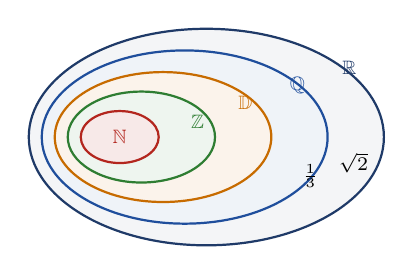
\begin{tikzpicture}[scale=0.55,font=\scriptsize]
\draw[cSec,thick,fill=cSec!5] (0,0) ellipse (4.1 and 2.5); \node[cSec] at (3.3,1.6){$\R$};
\draw[cDef,thick,fill=cDef!7] (-0.5,0) ellipse (3.3 and 2); \node[cDef] at (2.1,1.2){$\Q$};
\draw[cEx,thick,fill=cEx!8] (-1,0) ellipse (2.5 and 1.5); \node[cEx] at (0.9,0.8){$\D$};
\draw[cRem,thick,fill=cRem!8] (-1.5,0) ellipse (1.7 and 1.05); \node[cRem] at (-0.2,0.35){$\Z$};
\draw[cThm,thick,fill=cThm!10] (-2,0) ellipse (0.9 and 0.6); \node[cThm] at (-2,0){$\N$};
\node at (3.4,-0.6){$\sqrt2$}; \node at (2.4,-0.9){$\frac13$};
\end{tikzpicture}\end{LTR}}
\par\smallskip
\Lab{cRem}{ملاحظات}\par
\ck\ كل عدد ناطق له كتابة عشرية \textbf{منتهية} أو \textbf{دورية}: $\dfrac13=0{,}333\ldots$ ، $\dfrac{3}{11}=0{,}2727\ldots$\par
\ck\ نكتب $3\in\N$ ، $\frac23\notin\D$ ، $\R^{*}=\R-\{0\}$ ، $\R_{+}$ الأعداد الحقيقية الموجبة.
\par\smallskip
\Lab{cThm!80!black}{حذار}\ $3{,}14$ قيمة مقربة لـ $\pi$ وليست $\pi$ ؛ \ $\frac{22}{7}\in\Q$ لكن $\pi\notin\Q$.}{50 د}{تدوَّن التعاريف في الكراريس. يُرسم المخطط على السبورة ويُطلب من التلاميذ وضع أعداد النشاط فيه.}
\Row{التقويم}{%
\Lab{cEx}{تطبيق}\par
\Num{1} أكمل بـ $\in$ أو $\notin$: \ $-5\ldots\N$ ؛ $\frac{9}{3}\ldots\N$ ؛ $\frac{5}{6}\ldots\D$ ؛ $\sqrt{25}\ldots\Z$ ؛ $\frac{3}{8}\ldots\D$.\par
\Num{2} اكتب $x=0{,}3636\ldots$ على شكل كسر.\par
\textbf{الحل:} \Num{1} $\notin$ ؛ $\in$ ؛ $\notin$ ؛ $\in$ ؛ $\in$ (لأن $8=2^3$). \quad \Num{2} $100x-x=36$ ، إذن $x=\dfrac{36}{99}=\bx{\dfrac{4}{11}}$.\par
\textbf{واجب منزلي:} تمارين من الكتاب المدرسي حول مجموعات الأعداد.\par\smallskip\textbf{ملاحظات حول سير الحصة:} \dotfill}{25 د}{تقويم فردي على الألواح ، ثم تصحيح جماعي.}
\end{Sayr}
\newpage
\ModhHead{02}{1 ج م ع ت}{تحليل}{الأعداد والحساب}{02 سا}{الأعداد الأولية وتحليل عدد طبيعي إلى جداء عوامل أولية}%
{\begin{itemize}\item قواسم عدد طبيعي ومضاعفاته.\item قواعد قابلية القسمة على $2$ ، $3$ ، $5$ ، $9$.\end{itemize}}%
{\begin{itemize}\item التعرّف على أولية عدد طبيعي.\item تحليل عدد طبيعي إلى جداء عوامل أولية واستعماله.\end{itemize}}%
{المنهاج ، الكتاب المدرسي ، مراجع ، الحاسبة.}
\begin{Sayr}
\Row{مرحلة الانطلاق}{%
\textbf{التهيئة النفسية:} التذكير بقواعد قابلية القسمة.\par\Num{1} هل يقبل $1035$ القسمة على $3$ ؟ على $5$ ؟ \quad \Num{2} اكتب $36$ على شكل جداء بطرق مختلفة.}{10 د}{أسئلة شفهية سريعة.}
\Row{التشخيص والاكتشاف}{%
\Lab{cEx}{مناقشة نشاط 06 صفحة 3}\par\ck\ العدد الذي يقبل بالضبط قاسمين ($1$ ونفسه) هو عدد \textbf{أولي}: $2$ ، $3$ ، $5$ ، $7$ ، $11$ ، $13$ ، $\ldots$\par
\ck\ نشطب من جدول الأعداد من $2$ إلى $100$ مضاعفات $2$ ، ثم $3$ ، ثم $5$ ، ثم $7$: الأعداد الباقية هي الأعداد الأولية (\textbf{غربال إراتوستين}).\par
\ck\ نتوقف عند $7$ لأن $11^2=121>100$.\par
\ck\ العدد $1$ ليس أولياً لأن له قاسماً واحداً.\par
}{35 د}{يُوزَّع جدول الأعداد من $2$ إلى $100$ ؛ عمل ثنائي بالألوان.}
\Row{بناء المعارف}{%
\Lab{cDef}{تعريف}\ نقول عن عدد طبيعي $p$ إنه \textbf{أولي} إذا قبل بالضبط قاسمين مختلفين هما $1$ و $p$.\par\Lab{cThm}{خاصية}\ إذا لم يقبل $n$ ($n\geqslant2$) القسمة على أي عدد أولي $p$ يحقق $p^2\leqslant n$ فإن $n$ أولي.\par}{50 د}{نعرض القسمة المتتالية في عمود على السبورة.}
\Row{}{%
\Lab{cThm}{مبرهنة}\ كل عدد طبيعي $n\geqslant2$ يقبل تحليلاً \textbf{وحيداً} إلى جداء عوامل أولية.\par\Lab{cEx}{مثال -1-}\par\ck\ $97$ لا يقبل القسمة على $2$ ، $3$ ، $5$ ، $7$ و $11^2>97$ ، إذن $97$ أولي.\par
\ck\ $360=2^3\times3^2\times5$ (بالقسمات المتتالية على $2$ ، $2$ ، $2$ ، $3$ ، $3$ ، $5$).\par
}{}{}
\Row{}{%
\Lab{cMeth}{استعمالات التحليل}\par\ck\ اختزال كسر: $\dfrac{84}{126}=\dfrac{2^2\times3\times7}{2\times3^2\times7}=\dfrac23$.\par
\ck\ تبسيط جذر: $\sqrt{72}=\sqrt{2^2\times2\times3^2}=6\sqrt2$.\par
\Lab{cThm!80!black}{حذار}\ $91$ ليس أولياً رغم أنه فردي ولا يقبل القسمة على $3$: $91=7\times13$.}{}{}
\Row{التقويم}{%
\Lab{cEx}{تطبيق}\par\Num{1} حلّل $1176$ إلى جداء عوامل أولية. \ \Num{2} هل $221$ أولي؟ \ \Num{3} بسّط $\sqrt{1176}$.\par\textbf{الحل:} \Num{1} $1176=2^3\times3\times7^2$ ؛ \Num{2} $221=13\times17$ ليس أولياً ؛ \Num{3} $\sqrt{1176}=2\times7\sqrt{2\times3}=14\sqrt6$.\par\textbf{واجب منزلي:} تمارين من الكتاب المدرسي حول الأعداد الأولية.\par\smallskip\textbf{ملاحظات حول سير الحصة:} \dotfill}{25 د}{عمل فردي ثم تصحيح جماعي.}
\end{Sayr}
\newpage
\ModhHead{03}{1 ج م ع ت}{تحليل}{الأعداد والحساب}{02 سا}{البرهان بالخلف: $\sqrt2$ عدد أصم ، والأعداد القابلة للإنشاء}%
{\begin{itemize}\item مبرهنتا فيثاغورس وطالس.\item الأعداد الزوجية والفردية.\end{itemize}}%
{\begin{itemize}\item التمييز بين الأعداد الناطقة والصماء.\item البرهان بالخلف.\item إنشاء أعداد حقيقية بالمسطرة والمدور.\end{itemize}}%
{المنهاج ، الكتاب المدرسي ، أدوات الهندسة.}
\begin{Sayr}
\Row{مرحلة الانطلاق}{%
\textbf{التهيئة النفسية:} التذكير بمبرهنة فيثاغورس.\par\Num{1} الحاسبة تعطي $\sqrt2\approx1{,}414213562$ ، فهل $\sqrt2=\dfrac{1414213562}{10^9}$ ؟ \ \Num{2} احسب $(1{,}414213562)^2$ بالحاسبة.}{10 د}{نثير الشك في نتيجة الحاسبة.}
\Row{التشخيص والاكتشاف}{%
\Lab{cEx}{مناقشة النشاطين 02 و 03 صفحة 2}\par\ck\ قطر مربع ضلعه $1$ طوله $\sqrt{1^2+1^2}=\sqrt2$.\par
\ck\ وتر مثلث قائم ضلعاه $1$ و $2$ طوله $\sqrt5$ ؛ وبتكرار البناء نحصل على $\sqrt3$ ، $\sqrt4$ ، $\sqrt5$ ، $\ldots$ (\textbf{حلزون فيثاغورس}).\par
\ck\ بمبرهنة طالس نقسم قطعة إلى $3$ أجزاء متقايسة فنحصل على الطول $\dfrac23$.\par
\ck\ كل هذه الأعداد \textbf{قابلة للإنشاء} ؛ هل هي ناطقة؟\par
}{35 د}{عمل فردي بالأدوات الهندسية.}
\Row{بناء المعارف}{%
\Lab{cThm}{تمهيدية}\ إذا كان $p^2$ زوجياً فإن $p$ زوجي. (لأنه إذا كان $p=2k+1$ فإن $p^2=2(2k^2+2k)+1$ فردي.)\par\Lab{cMeth}{البرهان بالخلف}\ لنبرهن أن خاصية صحيحة ، نفرض أنها خاطئة ونصل إلى تناقض.\par}{50 د}{نكتب البرهان سطراً سطراً ونطلب تبرير كل سطر.}
\Row{}{%
\Lab{cThm}{خاصية}\ \bx{\sqrt2\notin\Q}.\par\textbf{البرهان:} نفرض $\sqrt2=\dfrac pq$ كسراً غير قابل للاختزال. إذن $p^2=2q^2$ ، فـ $p^2$ زوجي ومنه $p$ زوجي: $p=2k$. نعوّض: $4k^2=2q^2$ أي $q^2=2k^2$ ، فـ $q$ زوجي أيضاً. إذن $2$ يقسم $p$ و $q$ ، وهذا يناقض أن الكسر غير قابل للاختزال.\par\Lab{cRem}{ملاحظات}\par\ck\ العدد $\sqrt2$ \textbf{أصم} ، والعدد $1{,}414213562$ قيمة مقربة له فقط: مربعه لا يساوي $2$ تماماً.\par
\ck\ العدد القابل للإنشاء ليس بالضرورة ناطقاً.\par
}{}{}
\Row{التقويم}{%
\Lab{cEx}{تطبيق}\par\Num{1} برهن بالخلف أن $1+\sqrt2\notin\Q$. \ \Num{2} أنشئ قطعة طولها $\sqrt{10}$.\par\textbf{الحل:} \Num{1} لو كان $1+\sqrt2=r\in\Q$ لكان $\sqrt2=r-1\in\Q$: تناقض. \ \Num{2} وتر مثلث قائم ضلعاه $1$ و $3$.\par\textbf{واجب منزلي:} برهن أن $\sqrt3\notin\Q$ (اكتب $p=3k$ أو $p=3k+1$ أو $p=3k+2$).\par\smallskip\textbf{ملاحظات حول سير الحصة:} \dotfill}{25 د}{الواجب يُصحَّح في بداية الحصة القادمة.}
\end{Sayr}
\newpage
\ModhHead{04}{1 ج م ع ت}{تحليل}{الأعداد والحساب}{02 سا}{الحساب على الكسور والقوى الصحيحة ، الكتابة العلمية ورتبة المقدار}%
{\begin{itemize}\item العمليات على الكسور.\item القوى ذات الأسس الطبيعية.\end{itemize}}%
{\begin{itemize}\item التحكم في الحساب على الكسور والقوى الصحيحة.\item الكتابة العلمية والقوى الصحيحة للعدد $10$.\item تحديد رتبة مقدار عدد.\end{itemize}}%
{المنهاج ، الكتاب المدرسي ، مراجع ، الحاسبة.}
\begin{Sayr}
\Row{مرحلة الانطلاق}{%
\textbf{التهيئة النفسية:} حساب ذهني: $2^3\times2^2$ ؛ $\dfrac{10^5}{10^2}$ ؛ $\dfrac12+\dfrac13$ ؛ $\dfrac23\times\dfrac94$.}{10 د}{تذكير سريع.}
\Row{التشخيص والاكتشاف}{%
\Lab{cEx}{وضعية مقترحة}\par\Num{1} احسب $A=\Big(\dfrac23-\dfrac56\Big)\div\dfrac14$. \ \Num{2} احسب $B=\dfrac{2^3\times4^{-2}}{8^{-1}}$. \ \Num{3} المسافة بين الأرض والشمس حوالي $150\,000\,000$ km: كيف نكتبها باختصار؟\par\ck\ $A=\Big(\dfrac46-\dfrac56\Big)\times4=-\dfrac16\times4=\bx{-\dfrac23}$.\par
\ck\ $4^{-2}=\dfrac1{16}$ و $8^{-1}=\dfrac18$ ، إذن $B=\dfrac{8}{16}\times8=\bx{4}$.\par
\ck\ $150\,000\,000=1{,}5\times10^{8}$ km.\par
}{35 د}{نترك التلاميذ يكتشفون معنى الأس السالب.}
\Row{بناء المعارف}{%
\Lab{cThm}{قواعد الحساب على الكسور}\ $\dfrac ab+\dfrac cd=\dfrac{ad+bc}{bd}$ ؛ $\dfrac ab\times\dfrac cd=\dfrac{ac}{bd}$ ؛ $\dfrac ab\div\dfrac cd=\dfrac ab\times\dfrac dc$.\par\Lab{cDef}{تعريف}\ من أجل $a\ne0$ و $n\in\N^*$: $a^{-n}=\dfrac1{a^n}$ و $a^0=1$.\par}{50 د}{نكتب كل الأعداد بنفس الأساس ؛ نلخص القواعد في جدول.}
\Row{}{%
\Lab{cThm}{قواعد القوى}\ من أجل $m,n\in\Z$: $a^m\times a^n=a^{m+n}$ ، $\dfrac{a^m}{a^n}=a^{m-n}$ ، $(a^m)^n=a^{mn}$ ، $(ab)^n=a^nb^n$.\par\Lab{cDef}{الكتابة العلمية}\ كل عدد عشري موجب يُكتب $a\times10^{n}$ حيث $1\leqslant a<10$ و $n\in\Z$.\par}{}{}
\Row{}{%
\Lab{cEx}{مثال}\par\ck\ $C=\dfrac{3^2\times9^{-3}\times27^2}{3^{-1}}=\dfrac{3^2\times3^{-6}\times3^{6}}{3^{-1}}=3^{3}=27$.\par
\ck\ $0{,}000042=4{,}2\times10^{-5}$ ؛ $345000=3{,}45\times10^5$.\par
\ck\ \textbf{رتبة مقدار:} $(3{,}1\times10^4)\times(2{,}2\times10^{-2})\approx3\times2\times10^2=6\times10^2$.\par
\Lab{cThm!80!black}{حذار}\ $4^{-2}\ne-16$ ؛ و $2^3\times3^2\ne6^5$.}{}{}
\Row{التقويم}{%
\Lab{cEx}{تطبيق}\par\Num{1} احسب $D=\dfrac{5^{-2}\times25^3}{125}$. \ \Num{2} اكتب بالكتابة العلمية: $0{,}00305$ و $72\times10^{4}$.\par\textbf{الحل:} \Num{1} $D=5^{-2}\times5^{6}\times5^{-3}=5$ ؛ \Num{2} $3{,}05\times10^{-3}$ و $7{,}2\times10^{5}$.\par\textbf{واجب منزلي:} تمارين من الكتاب المدرسي حول القوى.\par\smallskip\textbf{ملاحظات حول سير الحصة:} \dotfill}{25 د}{تقويم فردي.}
\end{Sayr}
\newpage
\ModhHead{05}{1 ج م ع ت}{تحليل}{الأعداد والحساب}{02 سا}{الجذور التربيعية والحساب المضبوط}%
{\begin{itemize}\item تعريف الجذر التربيعي لعدد موجب.\item المتطابقات الشهيرة.\end{itemize}}%
{\begin{itemize}\item التحكم في الحساب على الجذور التربيعية.\item التمييز بين القيمة المضبوطة والقيمة المقربة.\end{itemize}}%
{المنهاج ، الكتاب المدرسي ، مراجع ، الحاسبة.}
\begin{Sayr}
\Row{مرحلة الانطلاق}{%
\textbf{التهيئة النفسية:} \Num{1} هل $\sqrt9+\sqrt{16}=\sqrt{25}$ ؟ \ \Num{2} احسب $\sqrt{4\times9}$ و $\sqrt4\times\sqrt9$.}{10 د}{نسجل الخطأ الشائع على السبورة.}
\Row{التشخيص والاكتشاف}{%
\Lab{cEx}{مناقشة نشاط 04 صفحة 3}\par\ck\ بالقيم المقربة تعطي الحاسبة نتائج «قريبة» فقط ، ولا تسمح بالبرهان على مساواة.\par
\ck\ بالحساب المضبوط: $(\sqrt2+1)(\sqrt2-1)=(\sqrt2)^2-1^2=2-1=\bx{1}$.\par
\ck\ نستنتج: \textbf{في البرهان نستعمل الحساب المضبوط} ، والقيم المقربة للتقدير فقط.\par
}{35 د}{مقارنة نتائج الحاسبة بالحساب المضبوط.}
\Row{بناء المعارف}{%
\Lab{cThm}{خاصية}\ من أجل $a\geqslant0$ و $b\geqslant0$: $\sqrt{ab}=\sqrt a\times\sqrt b$ ؛ $\sqrt{\dfrac ab}=\dfrac{\sqrt a}{\sqrt b}$ ($b\ne0$) ؛ $(\sqrt a)^2=a$.\par\Lab{cThm}{خاصية}\ من أجل كل عدد حقيقي $a$: \bx{\sqrt{a^2}=|a|}.\par}{50 د}{نستعمل التحليل إلى عوامل أولية للتبسيط.}
\Row{}{%
\Lab{cThm!80!black}{حذار}\ $\sqrt{a+b}\ne\sqrt a+\sqrt b$ في الحالة العامة: $\sqrt{9+16}=5$ بينما $\sqrt9+\sqrt{16}=7$.\par\Lab{cEx}{مثال}\par\ck\ $\sqrt{50}=\sqrt{25\times2}=5\sqrt2$ ؛ $\sqrt{12}+\sqrt{27}=2\sqrt3+3\sqrt3=5\sqrt3$.\par
}{}{}
\Row{}{%
\Lab{cMeth}{إزالة الجذر من المقام}\ نضرب البسط والمقام في المرافق: $\dfrac{1}{\sqrt3-1}=\dfrac{\sqrt3+1}{(\sqrt3-1)(\sqrt3+1)}=\dfrac{\sqrt3+1}{2}$.}{}{}
\Row{التقويم}{%
\Lab{cEx}{تطبيق}\par بسّط: $A=\sqrt{75}-2\sqrt{12}+\sqrt3$ ؛ $B=(2-\sqrt3)(2+\sqrt3)$ ؛ $C=\dfrac{6}{\sqrt3}$.\par\textbf{الحل:} $A=5\sqrt3-4\sqrt3+\sqrt3=2\sqrt3$ ؛ $B=4-3=1$ ؛ $C=\dfrac{6\sqrt3}{3}=2\sqrt3$.\par\textbf{واجب منزلي:} تمارين من الكتاب المدرسي.\par\smallskip\textbf{ملاحظات حول سير الحصة:} \dotfill}{25 د}{تقويم فردي على الألواح.}
\end{Sayr}
\newpage
\ModhHead{06}{1 ج م ع ت}{تحليل}{الأعداد والحساب}{02 سا}{القيم المقربة ، التدوير والحاسبة العلمية}%
{\begin{itemize}\item الكتابة العشرية.\item الكتابة العلمية.\end{itemize}}%
{\begin{itemize}\item تدوير عدد عشري إلى $10^{-p}$.\item التمييز بين عدد وإحدى قيمه المقربة.\item استخدام الحاسبة العلمية لتنظيم وإجراء حساب.\end{itemize}}%
{المنهاج ، الكتاب المدرسي ، مراجع ، الحاسبة.}
\begin{Sayr}
\Row{مرحلة الانطلاق}{%
\textbf{التهيئة النفسية:} \Num{1} ما الرقم الذي يأتي بعد الفاصلة الثانية في $\pi$ ؟ \ \Num{2} هل $0{,}33=\dfrac13$ ؟}{10 د}{حوار شفهي.}
\Row{التشخيص والاكتشاف}{%
\Lab{cEx}{وضعية مقترحة}\par سعر قطعة قماش $\dfrac{1000}{3}$ DA. البائع يكتب $333{,}33$ DA ، وآخر يكتب $333{,}34$ DA. من على صواب؟\par\ck\ $\dfrac{1000}{3}=333{,}333\ldots$ لا تنتهي ، فكلا العددين \textbf{قيمة مقربة} وليس القيمة المضبوطة.\par
\ck\ $333{,}33$ قيمة مقربة بالنقصان ، و $333{,}34$ بالزيادة ، والتدوير إلى $10^{-2}$ يعطي $333{,}33$.\par
}{35 د}{وضعية من الحياة اليومية ؛ نقاش جماعي.}
\Row{بناء المعارف}{%
\Lab{cDef}{قيمة مقربة}\ إذا كان $a\leqslant x\leqslant b$ و $b-a=10^{-p}$ فإن $a$ قيمة مقربة لـ $x$ بالنقصان إلى $10^{-p}$ و $b$ بالزيادة.\par\Lab{cDef}{التدوير إلى $10^{-p}$}\ نأخذ القيمة المقربة (بالنقصان أو بالزيادة) الأقرب إلى $x$ ؛ إذا كان الرقم الموالي $5$ أو أكثر ندوّر بالزيادة.\par}{50 د}{نوضح استعمال الحاسبة خطوة خطوة.}
\Row{}{%
\Lab{cEx}{مثال}\par\ck\ $\pi\approx3{,}14$ ؛ $\dfrac23\approx0{,}67$ ؛ $\sqrt2\approx1{,}414$ (إلى $10^{-3}$).\par
\ck\ العدد $\dfrac23$ \textbf{قيمته المضبوطة} $\dfrac23$ ، و $0{,}67$ قيمة مقربة له.\par
\Lab{cMeth}{الحاسبة العلمية}\ نستعمل الأقواس للبسط والمقام: $\dfrac{1+\sqrt5}{2}\approx1{,}618$ ؛ ومفتاح $\times10^{x}$ للكتابة العلمية: $(2{,}5\times10^{-3})\times(4\times10^{6})=10^{4}$.\par}{}{}
\Row{}{%
\Lab{cThm!80!black}{حذار}\ الحاسبة تعرض قيمة مقربة: $\sqrt2\times\sqrt2$ قد يظهر $1{,}9999999$ على بعض الحاسبات.}{}{}
\Row{التقويم}{%
\Lab{cEx}{تطبيق}\par\Num{1} دوّر $12{,}3456$ إلى $10^{-2}$ و $10^{-3}$. \ \Num{2} أعط قيمة مقربة بالنقصان إلى $10^{-2}$ لـ $\dfrac{22}{7}$.\par\textbf{الحل:} \Num{1} $12{,}35$ و $12{,}346$ ؛ \Num{2} $\dfrac{22}{7}=3{,}1428\ldots$ ، إذن $3{,}14$.\par\textbf{واجب منزلي:} تمارين من الكتاب المدرسي.\par\smallskip\textbf{ملاحظات حول سير الحصة:} \dotfill}{25 د}{تقويم فردي.}
\end{Sayr}
\newpage
\ModhHead{07}{1 ج م ع ت}{تحليل}{الأعداد والحساب}{02 سا}{المقارنة والترتيب في $\R$}%
{\begin{itemize}\item العمليات على الأعداد الحقيقية.\item المتطابقات الشهيرة.\end{itemize}}%
{\begin{itemize}\item اختيار معيار لمقارنة عددين.\item استعمال خواص الترتيب والعمليات.\end{itemize}}%
{المنهاج ، الكتاب المدرسي ، مراجع ، الحاسبة.}
\begin{Sayr}
\Row{مرحلة الانطلاق}{%
\textbf{التهيئة النفسية:} \Num{1} رتّب: $\dfrac37$ ، $\dfrac49$ ، $0{,}43$. \ \Num{2} كيف تتأكد من الترتيب دون حاسبة؟}{10 د}{نجمع اقتراحات التلاميذ.}
\Row{التشخيص والاكتشاف}{%
\Lab{cEx}{مناقشة النشاطين 01 و 02 صفحة 25}\par\ck\ لمقارنة مساحتين أو محيطين نحسب \textbf{الفرق} ونحدد إشارته.\par
\ck\ قارن $A=\sqrt3+\sqrt5$ و $B=\sqrt2+\sqrt6$: $A^2=8+2\sqrt{15}$ و $B^2=8+2\sqrt{12}$ ، ومنه $A^2>B^2$ ، والعددان موجبان فـ $A>B$.\par
}{35 د}{عمل ثنائي.}
\Row{بناء المعارف}{%
\Lab{cDef}{تعريف}\ $a<b$ معناه $a-b<0$ (\textbf{معيار الفرق}).\par\Lab{cThm}{خواص الترتيب والعمليات}\par\ck\ $a<b\Rightarrow a+c<b+c$.\par
\ck\ إذا كان $c>0$: $a<b\Rightarrow ac<bc$ ؛ إذا كان $c<0$: $a<b\Rightarrow ac>bc$.\par
\ck\ من أجل $0<a<b$: $a^2<b^2$ ، $\sqrt a<\sqrt b$ ، $\dfrac1a>\dfrac1b$.\par
}{50 د}{نلخص الخواص في جدول.}
\Row{}{%
\Lab{cMeth}{مقارنة عددين}\ ندرس إشارة الفرق ، أو نقارن المربعين (لعددين موجبين) ، أو نقارن النسبة بـ $1$ (لعددين موجبين).\par\Lab{cEx}{مثال}\ $x=\dfrac{n}{n+1}$ و $y=\dfrac{n+1}{n+2}$: $x-y=\dfrac{n(n+2)-(n+1)^2}{(n+1)(n+2)}=\dfrac{-1}{(n+1)(n+2)}<0$ ، إذن $x<y$.\par}{}{}
\Row{}{%
\Lab{cThm!80!black}{حذار}\ عند الضرب في عدد سالب تنعكس المتباينة.}{}{}
\Row{التقويم}{%
\Lab{cEx}{تطبيق}\par قارن: \Num{1} $\dfrac37$ و $\dfrac49$ ؛ \Num{2} $2\sqrt3$ و $3\sqrt2$.\par\textbf{الحل:} \Num{1} $3\times9=27<28=4\times7$ إذن $\dfrac37<\dfrac49$ ؛ \Num{2} $(2\sqrt3)^2=12<18=(3\sqrt2)^2$ إذن $2\sqrt3<3\sqrt2$.\par\textbf{واجب منزلي:} تمارين من الكتاب المدرسي.\par\smallskip\textbf{ملاحظات حول سير الحصة:} \dotfill}{25 د}{تقويم فردي.}
\end{Sayr}
\newpage
\ModhHead{08}{1 ج م ع ت}{تحليل}{الأعداد والحساب}{02 سا}{الحصر والقيم المقربة}%
{\begin{itemize}\item خواص الترتيب والعمليات.\item التدوير.\end{itemize}}%
{\begin{itemize}\item حصر عدد حقيقي.\item حصر مجموع وفرق وجداء ومقلوب ونسبة.\item حصر عبارة جبرية.\end{itemize}}%
{المنهاج ، الكتاب المدرسي ، مراجع ، الحاسبة.}
\begin{Sayr}
\Row{مرحلة الانطلاق}{%
\textbf{التهيئة النفسية:} نعلم أن $1{,}41<\sqrt2<1{,}42$ و $1{,}73<\sqrt3<1{,}74$. ماذا نستنتج عن $\sqrt2+\sqrt3$ ؟}{10 د}{دون حاسبة.}
\Row{التشخيص والاكتشاف}{%
\Lab{cEx}{مناقشة نشاط 03 صفحة 25}\par\ck\ $3{,}14<\sqrt2+\sqrt3<3{,}16$: نجمع الحدود طرفاً بطرف.\par
\ck\ $-1{,}42<-\sqrt2<-1{,}41$ ، إذن $0{,}31<\sqrt3-\sqrt2<0{,}33$.\par
\ck\ $2{,}4393<\sqrt6<2{,}4708$: نضرب حدوداً موجبة.\par
\ck\ $\dfrac{1}{1{,}42}<\dfrac{1}{\sqrt2}<\dfrac1{1{,}41}$ ، أي $0{,}704<\dfrac1{\sqrt2}<0{,}710$.\par
}{35 د}{عمل ثنائي ؛ نرصد خطأ طرح الحدود.}
\Row{بناء المعارف}{%
\Lab{cThm}{خاصية}\ إذا كان $a<x<b$ و $c<y<d$:\par\ck\ $a+c<x+y<b+d$ ؛ $a-d<x-y<b-c$.\par
\ck\ إذا كانت الحدود موجبة: $ac<xy<bd$ ؛ $\dfrac1b<\dfrac1x<\dfrac1a$ ؛ $\dfrac ad<\dfrac xy<\dfrac bc$.\par
\Lab{cDef}{سعة الحصر}\ العدد $b-a$ ، وكلما صغرت كان الحصر أدق.\par}{50 د}{تُدوَّن القواعد.}
\Row{}{%
\Lab{cEx}{حصر عبارة}\ إذا كان $x\in[1;2]$: $2x-3\in[-1;1]$ ؛ $x^2\in[1;4]$ ؛ $\dfrac{1}{x+1}\in\Big[\dfrac13;\dfrac12\Big]$.\par\Lab{cThm!80!black}{حذار}\ لا نطرح الحدود ولا نقسمها مباشرة.}{}{}
\Row{التقويم}{%
\Lab{cEx}{تطبيق}\par $2<x<3$ و $1<y<2$. احصر $x+y$ ، $x-y$ ، $xy$ ، $\dfrac xy$.\par\textbf{الحل:} $3<x+y<5$ ؛ $0<x-y<2$ ؛ $2<xy<6$ ؛ $1<\dfrac xy<3$.\par\textbf{واجب منزلي:} تمارين من الكتاب المدرسي.\par\smallskip\textbf{ملاحظات حول سير الحصة:} \dotfill}{25 د}{تقويم فردي.}
\end{Sayr}
\newpage
\ModhHead{09}{1 ج م ع ت}{تحليل}{الأعداد والحساب}{02 سا}{المجالات: التمثيل ، التقاطع والاتحاد}%
{\begin{itemize}\item المتباينات والمستقيم العددي.\end{itemize}}%
{\begin{itemize}\item التعبير عن جزء متصل من $\R$ بمجال.\item تعيين تقاطع واتحاد مجالين.\end{itemize}}%
{المنهاج ، الكتاب المدرسي ، السبورة.}
\begin{Sayr}
\Row{مرحلة الانطلاق}{%
\textbf{التهيئة النفسية:} مثّل على المستقيم العددي الأعداد $x$ حيث $-1<x\leqslant4$.}{10 د}{عمل فردي.}
\Row{التشخيص والاكتشاف}{%
\Lab{cEx}{وضعية مقترحة}\par مثّل على نفس المستقيم: $A$: $-2\leqslant x\leqslant3$ و $B$: $1<x\leqslant5$ ، ثم لوّن الأعداد المشتركة ، ثم الأعداد التي تنتمي إلى أحدهما على الأقل.\par\ck\ المشترك: $]1;3]$ ؛ أحدهما على الأقل: $[-2;5]$.\par
}{35 د}{نستعمل الألوان على المستقيم العددي.}
\Row{بناء المعارف}{%
\Lab{cDef}{تعريف}\par\ck\ المجالات المحدودة: $[a;b]$ ، $]a;b[$ ، $[a;b[$ ، $]a;b]$.\par
\ck\ غير المحدودة: $[a;+\infty[$ ، $]a;+\infty[$ ، $]-\infty;b]$ ، $]-\infty;b[$ ، و $\R=]-\infty;+\infty[$.\par
\Lab{cDef}{التقاطع والاتحاد}\ $I\cap J$: الأعداد التي تنتمي إلى $I$ \textbf{و} $J$ ؛ $I\cup J$: التي تنتمي إلى $I$ \textbf{أو} $J$.\par}{50 د}{نرسم جدول التوافق: متباينة ، مجال ، تمثيل.}
\Row{}{%
\Lab{cEx}{مثال}\ $[-2;3]\cap]1;5]=]1;3]$ ؛ $[-2;3]\cup]1;5]=[-2;5]$ ؛ $]-\infty;1[\cap[4;+\infty[=\varnothing$.\par\Lab{cThm!80!black}{حذار}\ الرمز $\infty$ ليس عدداً ، فالقوس عنده مفتوح دائماً.}{}{}
\Row{التقويم}{%
\Lab{cEx}{تطبيق}\par اكتب بمجال: $-1<x\leqslant4$ ؛ $x\geqslant2$. عيّن $]-3;2]\cap[0;5[$ و $]-3;2]\cup[0;5[$.\par\textbf{الحل:} $]-1;4]$ ؛ $[2;+\infty[$ ؛ $[0;2]$ ؛ $]-3;5[$.\par\textbf{واجب منزلي:} تمارين من الكتاب المدرسي.\par\smallskip\textbf{ملاحظات حول سير الحصة:} \dotfill}{25 د}{تقويم فردي.}
\end{Sayr}
\newpage
\ModhHead{10}{1 ج م ع ت}{تحليل}{الأعداد والحساب}{02 سا}{القيمة المطلقة والمسافة}%
{\begin{itemize}\item المستقيم العددي والمجالات.\end{itemize}}%
{\begin{itemize}\item كتابة عبارة بقيمة مطلقة دون الرمز.\item التعبير عن مجال بأربع صيغ: مجال ، حصر ، مسافة ، قيمة مطلقة.\end{itemize}}%
{المنهاج ، الكتاب المدرسي ، السبورة.}
\begin{Sayr}
\Row{مرحلة الانطلاق}{%
\textbf{التهيئة النفسية:} ما المسافة بين النقطتين اللتين فاصلتاهما $-2$ و $5$ على المستقيم العددي؟ وبين $5$ و $-2$ ؟}{10 د}{المسافة موجبة دائماً.}
\Row{التشخيص والاكتشاف}{%
\Lab{cEx}{مناقشة نشاط 04 صفحة 25}\par\ck\ المسافة بين نقطتين فاصلتاهما $a$ و $b$ هي $b-a$ إذا كان $a\leqslant b$ ، و $a-b$ إذا كان $b\leqslant a$: نرمز لها $|a-b|$.\par
\ck\ الأعداد التي تبعد عن $3$ بأقل من $2$ أو تساوي $2$: $1\leqslant x\leqslant5$.\par
}{35 د}{عمل ثنائي على المستقيم العددي.}
\Row{بناء المعارف}{%
\Lab{cDef}{تعريف}\ $|x|=x$ إذا كان $x\geqslant0$ ، و $|x|=-x$ إذا كان $x\leqslant0$. \ المسافة بين $a$ و $b$: $|a-b|=|b-a|$.\par\Lab{cThm}{خاصية}\ $|xy|=|x|\,|y|$ ؛ $\sqrt{x^2}=|x|$ ؛ $|x+y|\leqslant|x|+|y|$.\par}{50 د}{نلخص الصيغ الأربع في جدول.}
\Row{}{%
\Lab{cThm}{الصيغ الأربع}\ من أجل $r>0$: \ $|x-a|\leqslant r\iff a-r\leqslant x\leqslant a+r\iff x\in[a-r;a+r]$ ، أي: $x$ يبعد عن $a$ بـ $r$ على الأكثر.\par\Lab{cEx}{مثال}\par\ck\ $|\sqrt2-2|=2-\sqrt2$ لأن $\sqrt2<2$.\par
\ck\ المجال $[-1;7]$ مركزه $3$ ونصف قطره $4$: $x\in[-1;7]\iff|x-3|\leqslant4$.\par
}{}{}
\Row{}{%
\Lab{cThm!80!black}{حذار}\ $|-x|$ لا يساوي $x$ دائماً: $|-x|=|x|$.}{}{}
\Row{التقويم}{%
\Lab{cEx}{تطبيق}\par\Num{1} اكتب بمجال: $|x+1|<3$. \ \Num{2} اكتب $[2;8]$ بقيمة مطلقة. \ \Num{3} اكتب $|\pi-4|$ دون الرمز.\par\textbf{الحل:} \Num{1} $]-4;2[$ ؛ \Num{2} $|x-5|\leqslant3$ ؛ \Num{3} $4-\pi$.\par\textbf{واجب منزلي:} تمارين من الكتاب المدرسي.\par\smallskip\textbf{ملاحظات حول سير الحصة:} \dotfill}{25 د}{تقويم فردي.}
\end{Sayr}
\newpage
\ModhHead{11}{1 ج م ع ت}{تحليل}{الأعداد والحساب}{02 سا}{معادلات ومتراجحات بقيمة مطلقة ، البرهان بفصل الحالات ، إشارة ثنائي حد}%
{\begin{itemize}\item القيمة المطلقة والمسافة.\item حل معادلة ومتراجحة من الدرجة الأولى.\end{itemize}}%
{\begin{itemize}\item حل معادلات ومتراجحات بقيمة مطلقة.\item البرهان بفصل الحالات.\item تعيين إشارة ثنائي حد $ax+b$.\end{itemize}}%
{المنهاج ، الكتاب المدرسي ، السبورة.}
\begin{Sayr}
\Row{مرحلة الانطلاق}{%
\textbf{التهيئة النفسية:} ما الأعداد التي تبعد عن $2$ بمسافة $3$ ؟ ومتى يكون $-2x+6$ موجباً؟}{10 د}{ربط بالحصة السابقة.}
\Row{التشخيص والاكتشاف}{%
\Lab{cEx}{وضعية مقترحة}\par حل: \Num{1} $|x-2|=3$ ؛ \Num{2} $|x+1|=|x-3|$ ؛ \Num{3} $|2x-1|\leqslant5$.\par\ck\ $|x-2|=3\iff x=5$ أو $x=-1$.\par
\ck\ $x$ على نفس البعد من $-1$ و $3$ ، إذن $x=1$ (منتصف المجال).\par
\ck\ $-5\leqslant2x-1\leqslant5\iff-2\leqslant x\leqslant3$.\par
}{35 د}{نعرض طريقتي المسافة والحساب.}
\Row{بناء المعارف}{%
\Lab{cThm}{خاصية}\ من أجل $r>0$: $|X|=r\iff X=\pm r$ ؛ $|X|\leqslant r\iff-r\leqslant X\leqslant r$ ؛ $|X|>r\iff X<-r$ أو $X>r$.\par\Lab{cMeth}{البرهان بفصل الحالات}\ لكتابة $f(x)=|x-1|+|x+2|$ دون الرمز ندرس الحالات: $x\leqslant-2$: $f(x)=-2x-1$ ؛ $-2\leqslant x\leqslant1$: $f(x)=3$ ؛ $x\geqslant1$: $f(x)=2x+1$.\par}{50 د}{نرسم جدول الإشارة لكل عامل.}
\Row{}{%
\Lab{cThm}{إشارة ثنائي حد}\ $ax+b$ ($a\ne0$) ينعدم عند $-\dfrac ba$ ، وإشارته إشارة $a$ على يمين جذره وعكسها على يساره:\par\smallskip\begin{LTR}\centering\renewcommand{\arraystretch}{1.4}
\begin{tabular}{|c|ccccc|}\hline
\rowcolor{cSec!12}$x$ & $-\infty$ & & $-\frac ba$ & & $+\infty$\\\hline
$ax+b$ & & \ar{عكس إشارة $a$} & $0$ & \ar{إشارة $a$} & \\\hline
\end{tabular}\end{LTR}\par\Lab{cEx}{مثال}\ حل $(x-1)(3-x)>0$: بجدول الإشارة $S=]1;3[$.}{}{}
\Row{التقويم}{%
\Lab{cEx}{تطبيق}\par حل: \Num{1} $|x+2|=4$ ؛ \Num{2} $|2x+3|\geqslant1$ ؛ \Num{3} $(x+2)(1-2x)\geqslant0$.\par\textbf{الحل:} \Num{1} $\{-6;2\}$ ؛ \Num{2} $]-\infty;-2]\cup[-1;+\infty[$ ؛ \Num{3} $\Big[-2;\dfrac12\Big]$.\par\textbf{واجب منزلي:} تمارين حوصلة المحور من الكتاب المدرسي.\par\smallskip\textbf{ملاحظات حول سير الحصة:} \dotfill}{25 د}{نهاية المحور: فرض أو تمارين حوصلة.}
\end{Sayr}
\end{document}
